\documentclass[a4paper,11pt]{article}
\usepackage[T1]{fontenc} 
\usepackage{times}
\usepackage{a4wide}
\usepackage{amsthm, amsmath, amssymb}
\usepackage{algorithm}
\usepackage[noend]{algpseudocode}
\usepackage[british]{babel}
\usepackage{cases}
\usepackage{dsfont}
\usepackage{array}
\usepackage{chngcntr}
\usepackage{mathrsfs}
\usepackage{hyperref}
\usepackage[authoryear]{natbib}
\usepackage{fancyvrb}
\usepackage[normalem]{ulem} 
\usepackage{bbm}
\usepackage{bm}
\usepackage{latexsym}
%\usepackage{xcolor}
\usepackage[pdftex]{xcolor, graphicx}
\usepackage[normalem]{ulem}
\usepackage[font={small}]{caption}
\usepackage{lipsum}                    	
\usepackage{verbatim}
\usepackage{url}
\usepackage{authblk}

\usepackage{accents}

\newlength{\dhatheight}
\newcommand{\doublehat}[1]{%
    \settoheight{\dhatheight}{\ensuremath{\hat{#1}}}%
    \addtolength{\dhatheight}{-0.35ex}%
    \hat{\vphantom{\rule{1pt}{\dhatheight}}%
    \smash{\hat{#1}}}}

\newtheorem{theorem}{Theorem}
\makeatletter
\renewcommand\@biblabel[1]{-}
\makeatother
\theoremstyle{remark}
\newtheorem{remark}{Remark}

\newtheorem*{xmpl}{Example}
\theoremstyle{plain}
\newtheorem{corollary}{Corollary}
\newtheorem{lemma}{Lemma}
\newtheorem{assumption}{Assumption}
\newtheorem{definition}{Definition}
\newtheorem{proposition}{Proposition}
\def\argmax{\mathop{\rm argmax}}
\def\argmin{\mathop{\rm argmin}}
\newcommand\dotss{,\,\dots,\,}


\newcommand\ab[1]{{\color{blue} #1 }}

\usepackage{tikz}
\usepackage{stackengine}

\usetikzlibrary{arrows,positioning}


\title{Pair trading on Cryptocurrencies}

\author{Alessandro Balata\thanks{A.Balata@leeds.ac.uk} } 
\author{Jack Dry\thanks{jack\textunderscore dry@outlook.com}} 
\author{John McKenzie\thanks{jrm228@cam.ac.uk}} 
\author{Aliaksei Mikhailiuk\thanks{aliaksei.mikhailiuk@gmail.com}}

\affil{The Quant Group - \textit{www.thequantgroup.org} -}


\begin{document}

\maketitle

\begin{abstract}
In this paper we explore the idea of cointegration and its application to trading. We develop trading strategies for different currencies and provide back-tests that show the profit opportunities from implementing pair trading strategies on the cryptocurrency market.
\end{abstract}

\section{Introduction}

\ab{work on introduction}

Pairs trading is a strategy that was popularized in the 80's, which consists of simultaneously holding opposing positions in a pair of instruments, that are related in some statistical or fundamental way. A widespread notion of statistical relatedness is that of correlation, which focuses on the direction of movement in asset prices. In this sense, a pair trading strategy looks to profit from a temporary weakening of such correlation. Another notion of statistical relatedness is that of \textit{cointegration}, which identifies the degree to which asset prices move with respect to the same mean over some time period. Here, a pair trading strategy looks to profit from an eventual deviation from this mean.

While these strategies have been commonly employed in more traditional securities such as stocks, or ETFs, its application to novel instruments such as cryptocurrencies appears to be novel. In this sense, and given the direction-independent advantages of cointegration over correlation, we expect, among the many cryptocurrencies available today, to find groups of them that are highly cointegrated and share fundamental characteristics such as their technology, security, privacy, associated transaction costs, capitalization, liquidity and others. We would expect the price of these currencies to behave similarly, on average, opening opportunities for trading the spread in each pair within the groups.

The rest of the paper is organised as follow: in section \ref{sec:cointegration} we introduce the idea of cointegration and we highlight the most relevant aspects in building a trading strategy; in subsection \ref{sec:index} we explore a new notion of pair trading which we call index trading, and involve the  use of multiple currencies rather than just two. In section \ref{sec:cryptos} we introduce the market of cryptocurrencies and identify the coins we want to trade. Section \ref{sec:trading} gives a formal introduction of trading strategy on a stationary mean reverting process. The mathematics developed in the previous sections is finally applied to the coins identified in section \ref{sec:cryptos}, synthetic assets and trading strategies are computed and the performance of such strategies are computed on real data. 

\section{Cointegration and spread computation}
\label{sec:cointegration}
The ideal situation for a trader is to identify an asset whose price process is stationary and mean reverting. For the lucky investor profitable trading on this asset is almost sure, provided she has enough time to wait for the asset price to revert to its long term (constant and known) mean. The trading strategy is simple enough, buy low and sell high. Further, when the dynamics of the price process are exactly those of a OU process (or AR(1) in discrete time), optimal entry and exit points are known analytically.
In the real world however we struggle to find such assets, and even in the most promising situations, we can at best hope to find a mean reverting process with volatility clusters and stochastic long-term mean. In these conditions it is less clear whether the investor will be able to profit from simple trading strategies and rather she will need exogenous factors to predict changes in price volatility and the level of the long term mean.

\subsection{Simple OLS estimation}
\label{sub:simple_OLS}

An alternative approach which aims at retrieving the ideal situation presented at the beginning of the section is to construct a synthetic product (spread hereafter), that enjoys the properties of stationarity and mean reversion, using assets traded on the market. The mathematical concept of cointegration helps us to identify the assets underlying the spread.

More formally, assume for now that we are given two cointegrated time series $X^1$ and $X^2$, whose element at time $t$ are denoted by $X^i_t$, $i=1,2$. It is well known (\ab{add reference}) that it exists a linear combination of these time series $Y=b^1X^1+b^2X_2$ that is stationary and mean reverting. Assuming now that the resulting time series at time $t$, $Y_t$ is normally distributed, we can compute the coefficients $b^1$ and $b^2$ rewriting:
\begin{equation}
\label{eq:ols}
Y=b^1X^1+b^2X_2\;\Rightarrow\;X^1=-\frac{b_2}{b_1}X^2+\frac{1}{b_1}Y=\beta^0+\beta X^2+\hat{Y},
\end{equation}
where w.l.o.g. we fix $b_1=1$ and denote $\beta=-b_2$, $\beta^0=\mathbb{E}[Y]$ and $\hat{Y}=Y-\mathbb{E}[Y]$. We can notice from \eqref{eq:ols} that as long as $\hat{Y}_t\sim\mathcal{N}(0,\sigma)$, OLS estimation of $(\beta^0,\beta)$ is a viable approach. 
It should be noted however that if all assumptions were satisfied, the sequence $\{Y_s\}_{s=0}^T$ should be $i.i.d.$, $\forall\,T$; such situation is never observed in practice, while it is common to have some residual autocorrelation in the process $\hat{Y}$. From the point of view of the investor, however, this does not represent an insurmountable difficulty, as long as the properties of stationarity and mean reversion are preserved.

Denoting by $\boldsymbol{\beta}=(\beta^0,\beta)^T$ and $\boldsymbol{\phi}_s=(1, X^2_s)^T$, we can compute
\begin{equation}
\label{eq:simpleOLS}
\boldsymbol{\beta}=\text{arg}\min\limits_{b_0,b}\Big\{\frac{1}{T}\sum\limits_{s=1}^{T}\big(X_1-b_0-b X^2\big)^2 \Big\}=\frac{\mathcal{A}}{T\sum\limits_{s=1}^{T}(X^2_s)^2-\left(\sum\limits_{s=1}^{T}X^2_s\right)^2}\sum\limits_{s=1}^{T}X^1_s \boldsymbol{\phi}_s,
\end{equation}
where $\mathcal{A}$ is the matrix:
\[
\mathcal{A}=\left(\begin{bmatrix}
    1 & \dots & 1\\
    X^2_1 & \dots & X^2_T 
\end{bmatrix}
\begin{bmatrix}
    1 & X^2_1 \\
    \vdots & \vdots \\
     1 & X^2_T
\end{bmatrix}
\right)^{-1}=\begin{bmatrix}
     T & \sum_{s=1}^{T}X^2_s \\
    \sum_{s=1}^{T}X^2_s & \sum_{s=1}^{T}(X^2_s)^2
\end{bmatrix}^{-1}=\begin{bmatrix}
    \sum_{s=1}^{T}(X^2_s)^2 & - \sum_{s=1}^{T}X^2_s \\
    - \sum_{s=1}^{T}X^2_s & T
\end{bmatrix}
\]

Once we have computed the coefficients $\boldsymbol{\beta}$ we can write explicitly $Y=X^1-\beta X^2$ and provide the investor with a stationary mean reverting asset which can be traded as follow:
\begin{itemize}
\item When $Y$ is ``high'', we would like to short it $\Rightarrow$ we sell 1 unit of $X^1$ and buy $\beta$ units $X^2$
\item When $Y$ is ``low'', we would like to go long $\Rightarrow$ we buy 1 unit of $X^1$ and sell $\beta$ units $X^2$
\end{itemize}
Note that $\beta$ needs not to be positive, hence we could have situations in which we buy or sell both underlying assets.

\subsection{Rolling OLS estimation}
Even though the approach presented in the previous section convinced the investor to put some money into this strategy, she can not find a pair of assets $(X_1,X_2)$ cointegrated over the last $T$ days ( we skip for now the formal presentation of the statistical tests for cointegration and carry over with a more intuitive presentation of our heuristic approach). Even though it is not rigorous to talk about two series being loosely or closely cointegrated, we could suppose that in the real world we find only assets with a low level of cointegration and therefore we are not able to build any stationary, mean-reverting process $Y$ using the technique just described. In order to overcome this difficulty we can employ a widespread heuristic approach, the rolling OLS estimation. It should be understood, however, that a careful implementation of this technique is necessary as it may lead to strategies which can not be implemented in practice.

A rolling estimation of the coefficients $\boldsymbol{\beta}$ allows to have much greater flexibility in fitting the series $\{X^1\}_{s=1}^{T}$ using $\{X^2\}_{s=1}^{T}$ and works generally well in practice. The implementation of this technique is equivalent to the simple OLS presented in the first section, in this case however we will estimate a time dependent vector of parameters as follow. Denote by $\boldsymbol{\beta}_s=(\beta^0_s, \beta_s)$ $s\in[W+1,T]$, where $W$ is width of the window we apply to the data. Compute the OLS estimation of $\boldsymbol{\beta}_s$ fitting $\{X^1_j\}$ with $\{\boldsymbol{\phi}_j\}$, $j\in[s-W,s]$.

The width of the window $W$ influences the sensitivity of $\beta$ to changes in the relation between the two underlying assets. A narrow window will be faster in detecting changes in the behaviour of the underlyings, but it will encode a lot of noise in the value of $\beta$; on the other hand wide windows will produce smoother maps $s\mapsto\beta_s$ which are more robust and, locally, justified by section \ref{sub:simple_OLS}.

Notice that, heuristically, we would expect to find a qualitatively close resemblance between the graphs of $s\mapsto X^1_s$ and $s\mapsto \beta^0_s+\beta_s X^2_s$. We can further standardize, under the usual assumption of normality, the value of $Y$ by computing $Z_s=\frac{\hat{Y}_s}{\sigma_s}=\frac{Y_s-b^0_s}{\sigma_s}$. Under the standing assumption the random variable $Z_s\sim\mathcal{N}(0,1)$ allowing to devise standard trading strategies to be applied to many products built from pairs of underlying assets.

\subsection{Generalised index trading}
\label{sec:index}
We introduce in this section an heuristic approach developed on the basis of the general definition of cointegration. Consider a set of $N$ time series $(X^1,\,\dots,\,X^N)$ and define the process $Y$ as the linear combination:
\[
Y^N_s=\sum_{n=1}^{N}\beta^n_s X^n_s.
\]
If it exists at least a collection of vectors $\{\boldsymbol{\beta}_s\}_{s=W}^{T}$ such that $Y^N$ is stationary, then $(X^1,\,\dots,\,X^N)$ are said to be cointegrated.

If we can find a set of cointegrated assets to provide to an investor, she will be happy to invest in the group, rather than in the single pairs, as this will reduce the variance of the $P\&L$ of her trading strategy \ab{(this deserves more)}. 

By following the well known OLS estimation technique for multivariate regression, we can find the values of the coefficients $\{\beta_s^n\}_{s,n=1}^{T,N}$ and in turn implement a pair-trading strategy that enjoys the benefit of diversification.

\ab{(should be discussed: why its better to trade a spread among 3 assets rather than 2 pairs--- lower transaction cost? lower estimation error?) }

\subsection{Statistical tests}
 
\ab{In this section we should explain the statistical test used to verify cointegration}

\section{Trading Cryptocurrencies}
\label{sec:cryptos}

Different factors have lead us to the decision of applying the ideas presented in section \ref{sec:cointegration} to the cryptocurrencies market. The strong interest these assets are receiving from non-professional or semi-professional investors, along with the small proportion of professional investors participating in the market allows for profit opportunities which, on traditional markets, are nowadays available only to investors with access to dedicate, high performance, trading infrastructure. The small proportion of institutional investors in the cryptocurrency markets can be explained by a number of reasons spanning from the absence of regulation, the frequent hacks of coin wallets and the relatively small size of the market. The nature of this new asset class has also been paramount in the decision of looking for cointegration among coins. Being a young market, many coins are traded and only few have emerged as dominant. As long as this uncertainty about which coins will in turn survive the first phase of the market, we expect many similar alternatives to be traded at the same time. When referring to similar alternatives, we think of coins which have similar characteristics, as employing the same technology or serving the same purpose.

We reckon that grouping the coins by a fundamental analysis perspective should anticipate the statistical tests. The latter should be run only as mathematical verification rather than a searching tool, in order to avoid misuse of the $p$-values output by the test.

\subsection{Choice of the groups}

\ab{(this section is work in progress and should be updated as we get new results)}

Analysing the most capitalised cryptocurrencies on the market, we identified the following groups of coins showing clear economic reasons to have similar behaviour. Other less obvious cointegrated groups of coins might be available on the market, to limit the drawbacks of the iterative application of statistical tests however we limit ourselves to those we are able to justify by words.

It follows a description of the groups identified along with a list of the coin comprised in each group. Not all coins in a group need to be cointegrated, we expect and plan to consider only some of all possible pairing of coins within a group. 

\subsection{Payments-Anonymity-Security}
Many coins available today are aimed at providing a mean of payments that is secure, anonymous and cheap. In principle, the value of these coins should closely resemble the value of an imaginary representative coin and thus move randomly around a long term mean. This scenario, if confirmed by the statistical tests suggests that pair (or index) trading within this group could be profitable. 

\ab{the symbols showing the pairs considered are not updated; the other coins should be added too}

\begin{table}[h]
\centering
\begin{tabular}{l|lllll}
coins & \multicolumn{5}{l}{pairs} \\ \hline \hline
 Dash    &   x  &     &     &     &    \\  \hline
 Litecoin    &  x   &     &     &     &    \\  \hline
  Monero    &     &     &     &     &    \\  \hline
  PIVX   &     &    * &     &     &    \\  \hline
 Verge    &     &  *   &  $\dagger$   &     &    \\ \hline
 Vertcoin    &     &     &  $\dagger$   &     &    
\end{tabular}
\end{table}

\subsection{Smart Contracts and Services}
A third category under study comprises coins that offer services often robustly built around the blockchain infrastructure. A mentionable example of such coins selected for our study is represented by Siacoin, MaidSafeCoin and Storjcoin. These three coins allow you to buy online storage space, sold from other users that can profit from unused memory partitions on their hard drives. The services accessible by owning these coins are very similar, and most probably people selling space in one currency, do so in the others too. These characteristics clearly suggest that a test for cointegration is appropriate.

\begin{table}[h]
\centering
\begin{tabular}{l|lllll}
coins & \multicolumn{5}{l}{pairs} \\ \hline \hline
Ethereum     & x    &  *   &     &     &    \\ \hline
  NEO    &   x  &     &     &     &    \\ \hline
  IOTA    &     &  *   &     &     &    \\ \hline
  Siacoin    &     &     &  $\dagger$   &     &    \\ \hline
  MaidSafeCoin    &     &     &  $\dagger$   &     &    \\ \hline
   Storjcoin  &     &     &  $\dagger$   &     &   
\end{tabular}
\end{table}

\subsection{Forked}
Within this group we take into account the subgroups of coins generated by forking. Depending on the nature of the fork we could hypothesize that the price of the forked coin behave similarly to the price of the parent.

\begin{table}[h]
\centering
\begin{tabular}{l|lllll}
coins & \multicolumn{5}{l}{pairs} \\ \hline \hline
Bitcoin      &  x   &     &     &     &    \\ \hline
Bitcoin cash     & x    &     &     &     &    
\end{tabular}
\end{table}


\section{Trading strategy}
\label{sec:trading}


\section{Numerical results and Back-testing}
\label{sec:results}

\ab{this section should be updated as soon as ``decent results'' are available}

\section{\ab{old --> temporary}}

 \paragraph{Classification}
 
The idea is to find groups of cryptocurrencies, which share fundamental characteristics such as similar technologies, security, privacy, transaction cost, capitalization, etc. Next, we reconcile this with the cointegration notion of relatedness. For this purpose we follow the \textit{Engle-Granger} two step procedure.\footnote{In the future we would like to explore other cointegration test popularised by Johansen (1995)} This procedure consist of (i) identifying prices of cryptocurrencies which can be regarded as integrated processes of order $I(n)$ with $n\geq 1$. This can be done by repeatedly first-differencing and performing the \textit{ADF test of unit root} until we are confident that the price generating process looks stationary. Once that has been established, (ii) we proceed to determine the cointegrating relationship, which basically states that if $x_t$ and $y_t$ are integrated processes (both) of order $I(n)$ with $n \geq 1$, then a linear combination $x_t-\beta y_t$ may be stationary. This linear combination will be referred to as the spread.
 
 \paragraph{Spread Estimation:} We model the spread on a rolling basis and estimate the cointegrating parameters $\beta_t$ by OLS. We expect all spreads in a group to be modelled by the same process. 

 
 \paragraph{Optimal control / trading:} There are at least two alternatives: \ab{forecasting} Once we have models for the spread we can optimise the profits of trading on all the spreads searching for the best entry and exit points (within a finite time horizon over which we can construct a forecast of the spread). Such points should be refreshed in a rolling fashion, as new information arrives. In this way we can construct an online trading strategy.
 \ab{control policy} average performance infinite horizon stochastic optimization problem where you look for entry, stop loss and take profit levels.
 These strategy could be defined as ``offline'' as they do not need a real time supply of data to perform well (still to be refreshed  periodically ) 
 
 Once tradable pairs have been identified, we are left with a mean reverting processes and the task of finding optimal entry and exit points. Stop loss and profit taking levels should be defined in order to optimize the trade off between waiting that the spread reaches a level of statistical significance and entering immediately, in turn maximising the long term profits.

\subsection{Report}
In the past weeks we have analysed the top 100 cryptocurrencies by market capitalisation and existence in the market for at least a year. Then we selected a number of promising pairs satisfying the cointegration test. We believe that combining statistical and fundamental techniques would provide a solid selection criterion for the cryptocurrencies under consideration. We construct the spreads between elements of a pair via least square regression and moving average. An example of such procedure can be observed in Figure \ref{f:example}.

\subsection{Future work and timeline}
We are now directing our attention to the fine-tuning our spread estimation and developing the optimal control protocols that will ultimately define how to manage our positions in the cryptocurrencies. The expected timeline is as follow:

\begin{itemize}
\item[10/1/2018] Complete the whole procedure for one pair only to be able to carry over a backtest and provide a first assessment of the value of trading strategies constructed by following our methodology;
\item[20/1/2018] Extend estimation and optimal control to all the pairs selected in the classification step already completed;
\item[31/1/2018] Define clear trading strategies and backtest them on real and synthetic data
\item[28/2/2018] Complete the paper and submit for publication.
\end{itemize}

\begin{figure}
\centering
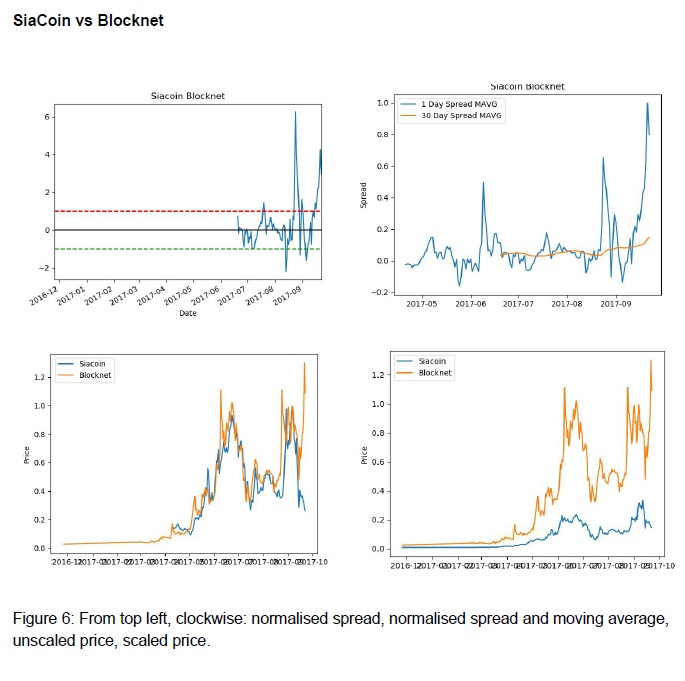
\includegraphics[scale=0.9742]{example.jpg}
\caption{Above an example of the procedure used to compute the normalised spread. The green and red lines in top left corner panel represent a naive training strategy with buy and sell levels placed at one standard deviation from the mean.} 
\label{f:example}
\end{figure}

\end{document}